\chapter{Suites numériques}

\label{chap:suite}
\section{Introduction~: Une histoire de lapins}
On considère des couples (inséparables) de lapins. Cette population évolue au fil des mois selon les règles suivantes~:
\begin{enumerate}
    \item Au début du premier mois, il y a un unique couple de lapins nouveau-nés.
    \item Au début de chaque nouveau mois, tout couple ayant vécu au moins 2 mois entiers donne naissance à un nouveau couple de bébés lapins.
    \item Les lapins sont immortels.
\end{enumerate}
L'image \ref{fig:rabbits} montre l'évolution des couples de lapins au fil des premiers mois.
\begin{figure}[H]
\centering 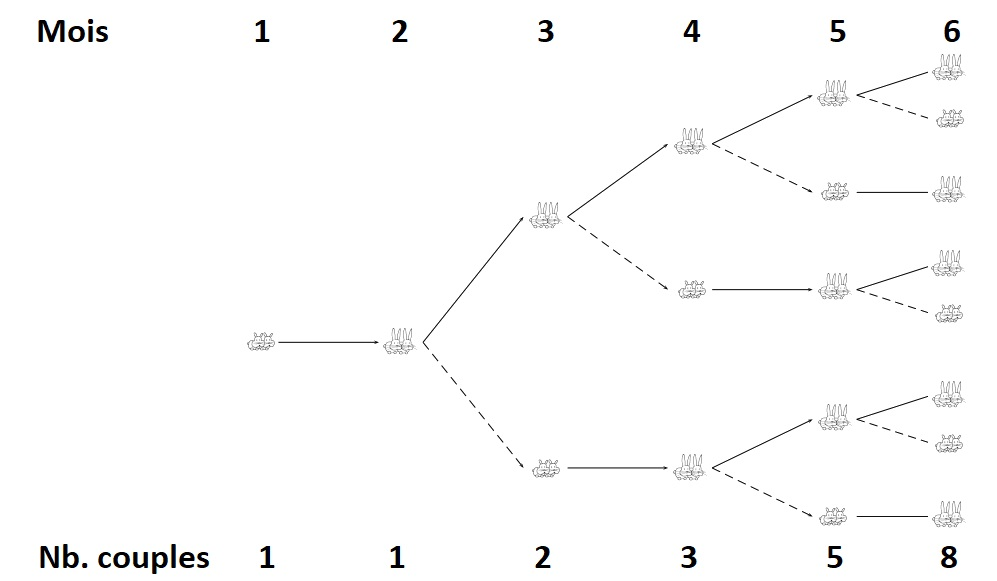
\includegraphics[width = 0.85\textwidth]{./assets/imgs/rabbit_tree.jpg}
\caption{Les couples de lapins au fil des 6 premiers mois}
\label{fig:rabbits}
\end{figure}

\begin{greybox}
\textbf{Question 1.} Combien de couples de lapins y a-t-il au mois numéro $n$ ? Ici, $n$ peut être n'importe quel nombre entier positif~: $n = 1, 2, 36, 1002,$ etc\textellipsis

On souhaite avoir une définition générale pour décrire le nombre de couples au $n$-ième mois, que l'on va dénoter $x_n$. 
\end{greybox}

\begin{boxdef}[Suite]
Une telle séquence de nombres réels $x_1, x_2, x_3, ...$, indexée par les entiers positifs de $\mathbb N$, est appelée \emph{suite}. On la note $(x_n)_{n \in \mathbb{N}^*}$, $(x_n)_{n \geq 1}$, ou simplement $(x_n)$, et on note $x_n$ le $n$-ième élément de la suite.
\label{def:suite}
\end{boxdef}

\begin{greybox}
\textbf{Question 2.} Quel est le comportement de $x_n$ quand $n$ devient grand ? Est-ce que $x_n$ devient très grand lui aussi ? Est-ce que $x_n$ oscille entre certaines valeurs ? Est-ce que $x_n$ se stabilise vers une valeur précise ? Ce sont quelques exemples de questions que l'on peut se poser lorsqu'on étudie une suite.
\end{greybox}

\begin{greybox}
\textbf{Question 3.} Quel est le nom de la suite décrite ci-dessus ?
\end{greybox}
On commence par répondre à la question 3~: il s'agit de la fameuse \emph{suite de Fibonacci}. 

Quant à la question 1, l'observation suivante est clé~: au mois numéro $n$, on a tous les couples de lapins du mois précédant ($x_{n-1}$ couples) + tous les couples qui viennent de naître. Seuls les couples déjà nés il y a au moins deux mois, soit $x_{n-2}$ couples, donnent naissance à un nouveau couple ! On a donc $$x_n = x_{n-1} + x_{n-2}, \quad n \geq 3$$ 
On doit se restreindre à $n \geq 3$ pour que cette formule soit bien définie (e.g. si on met $n = 2$, on obtient $x_2 = x_1 + x_0$, mais on n'a pas de mois numéro $0$ dans notre problème). Et par définition de notre problème, on a $x_1 = x_2 = 1$ (voir l'image \ref{fig:rabbits}), donc
\begin{equation}
    x_1 = x_2 = 1, \quad x_n = x_{n-1} + x_{n-2}, \quad n \geq 3
    \label{eq:fibonacci}
\end{equation}
ce qui définit tous les termes de la suite sans ambiguïté~: si on nous donne n'importe quel indice $n$, on peut calculer séquentiellement $x_3, x_4, ..., x_n$ en un temps fini grâce à la formule \ref{eq:fibonacci}.

Finalement, il reste à répondre à la question 2. Il découle de la formule \ref{eq:fibonacci} que si $x_{n-1}$ et $x_{n-2}$ sont $\geq 1$, alors $x_n = x_{n-1} + x_{n-2} \geq x_{n-1} + 1$. En partant de $x_1 = x_2 = 1$, on déduit que $(x_n)$ est une suite \emph{positive} ($x_n > 0$ pour tout $n$), \emph{croissante} ($x_n \geq x_{n-1}$ pour tout $n$) et \emph{non-bornée}~:
\begin{equation}
x_n \geq x_{n-1} + 1 \geq x_{n-2} + 1 + 1 \geq ... \geq x_2 + (n-2) = n-1
\label{eq:fibonacci_lower_bound}
\end{equation}

\begin{boxdef}[Suite bornée et non-bornée]
Une suite $(x_n)$ est dite \emph{bornée} si on peut l'encadrer par deux valeurs fixes, i.e. s'il existe un nombre réel $B > 0$ tel que $-B < x_n < B$ pour \textbf{tous} les indices $n$ ! On dit que la suite est \emph{non-bornée} si un tel nombre $B > 0$ n'existe \textbf{pas}. De manière équivalente, une suite est non-bornée si pour tout $B > 0$, on peut trouver au moins un indice $n$ tel que $|x_n| > B$ (c'est-à-dire $x_n < - B$ ou bien $x_n > B$).
\label{def:borné}
\end{boxdef}

\begin{figure}[H]
\centering 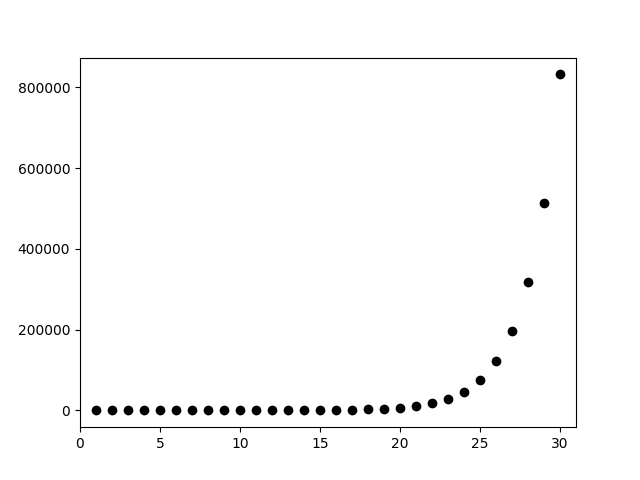
\includegraphics[width = 0.55\textwidth]{./assets/imgs/fibonacci.png}
\caption{Les 30 premières valeurs de la suite de Fibonacci}
\label{fig:fibonacci}
\end{figure}

Dans l'image \ref{fig:fibonacci}, on peut observer la croissance rapide de la suite de Fibonacci. Peu importe la ligne horizontale qu'on tracerait sur ce graphe, la suite va forcément la dépasser !

\section{Suites numériques}

Pour définir une suite, au sens de la Définition \ref{def:suite}, de manière rigoureuse, il y a 3 manières~:

\begin{enumerate}
    \item La suite est définie \emph{par récurrence}~: le $n$-ième élément $x_n$ est défini en fonction d'autres éléments $x_i$ avec des indices $i < n$. C'est le cas de la suite de Fibonacci étudiée précédemment~: $x_n = x_{n-1} + x_{n-2}$ pour $n \geq 3$ avec $x_1 = x_2 = 1$ comme point de départ. Il est important de bien donner les éléments initiaux de la suite, car ils ne peuvent pas être définis en termes d'autres éléments.
    \item La suite est définie explicitement~: le $n$-ième élément $x_n$ est une fonction de $n$. Par exemple, $x_n = n^2 + n - 2$ pour tout $n \geq 1$.
    \item La suite est définie par une propriété non-ambiguë~: par exemple, $x_n$ est le $n$-ième nombre premier.
\end{enumerate}

Les suites peuvent exhiber des propriétés diverses et variées. Il n'y a pas de règle générale permettant de décrire le comportement de toutes les suites en même temps. Voici néanmoins quelques exemples de comportements que l'on peut observer~:

\begin{enumerate}
    \item La suite de Fibonacci est croissante, non-bornée.
    \item La suite $x_n = (-1)^n$ est bornée, mais n'est ni croissante, ni décroissante. La suite alterne entre les valeurs $-1$ et $+1$.
    \item La suite $x_n = (-1)^n \cdot n$ est non-bornée, ni croissante, ni décroissante.
    \item La suite $x_n = \frac{1}{n}$ pour $n \geq 1$ est bornée car $-1 \leq x_n \leq 1$ pour tout $n \geq 1$, et elle est aussi décroissante.
\end{enumerate}

Étudions plus en détail le dernier exemple, $x_n = \frac{1}{n}$. Si on calcule les premiers termes explicitement, on observe le comportement suivant~: 

\begin{figure}[H]
\centering 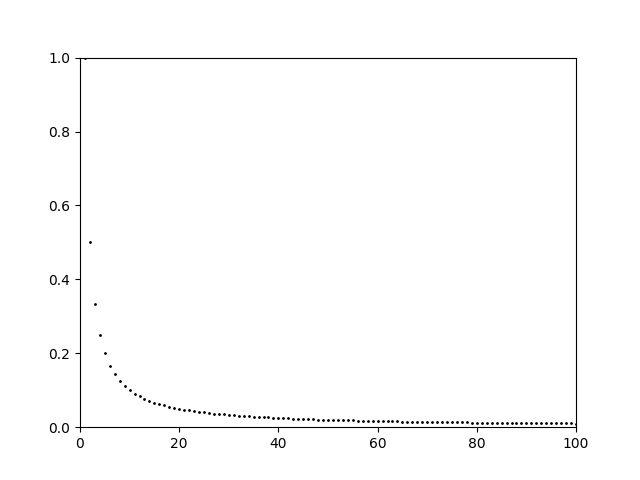
\includegraphics[width = 0.55\textwidth]{./assets/imgs/1_sur_n.png}
\caption{Les 100 premières valeurs de la suite $x_n = \frac{1}{n}$}
\label{fig:1_sur_n}
\end{figure}

On observe que plus $n$ devient grand, plus $\frac{1}{n}$ devient petit et se rapproche de $0$. Cela motive la définition (informelle) suivante~:

\begin{boxdef}[Convergence d'une suite (informelle)]
On dit qu'une suite $(x_n)_{n \geq 1}$ \emph{converge} vers un nombre $l \in \mathbb R$ si, en ignorant suffisamment de termes initiaux $x_1, x_2, ..., x_{n_0}$, \emph{tous} les éléments restants de la suite sont aussi proches de $l$ que l'on veut. On dit que $l$ est la \emph{limite} de la suite $(x_n)$ et on note 
\[
\lim \limits_{n \to \infty} x_n \eqdef l
\]

Si un tel nombre $l \in \mathbb R$ n'existe pas, on dit que la suite \emph{diverge}.
\label{def:convergence}
\end{boxdef}

Intuitivement, comme pour la suite $x_n = \frac{1}{n}$, cela signifie que lorsque $n$ est arbitrairement grand, $x_n$ devient arbitrairement proche de sa limite $l$ ($l = 0$ pour $x_n = \frac{1}{n}$). 

Reprenons à nouveau quelques exemples~:

\begin{enumerate}
    \item La suite de Fibonacci diverge. En effet, la propriété $x_n \geq n-1$ fait qu'on s'éloigne de plus en plus de n'importe quel nombre $l \in \mathbb R$ fixé lorsque $n$ augmente.
    \item La suite $x_n = (-1)^n$ diverge. En effet, on alterne toujours entre $-1$ et $+1$, mais la suite ne se stabilise jamais sur une des deux valeurs.
    \item La suite $x_n = \frac{n+2}{n+1} = 1 + \frac{1}{n+1}$ converge vers $1$.
    \item La suite $x_n = 1$ (suite constante) converge vers $1$.
\end{enumerate}

\section{Propriétés élémentaires des limites}

Avant toute chose, et même si cela peut paraître logique, il faut quand même se poser la question~: est-ce qu'une suite convergente $(x_n)$ peut avoir deux limites distinctes $l_1 \neq l_2$ ?

La réponse est non, c'est-à-dire que

\begin{boxthm}[Unicité de la limite]
La limite d'une suite convergente est \emph{unique}.
\end{boxthm}

En effet, lorsque $n$ devient très grand, la valeur $|x_n-l_1|$ (qui correspond à la distance entre $x_n$ et sa limite $l_1$) peut être rendue aussi proche de $0$ que l'on souhaite. De même, la valeur $|x_n-l_2|$  peut être rendue aussi proche de $0$ que l'on souhaite. On peut alors déduire que
$$|l_1 - l_2| = |(l_1 - x_n) + (x_n - l_2)| \leq |x_n - l_1| + |x_n - l_2| \quad \text{(inégalité triangulaire)}$$ peut être rendue aussi proche de $0$ que l'on souhaite, donc on a nécessairement $l_1 = l_2$.

Il découle également de notre définition informelle que 
\begin{boxthm}[Convergence implique borné]
Toute suite convergente est bornée.
\end{boxthm}

En effet, si $(x_n)$ converge vers $l \in \mathbb R$, alors on peut séparer la suite en des termes initiaux $x_1,x_2,...,x_{n_0}$ et le reste de la suite qui est très proche de $l$, disons au moins à distance $|x_n - l| \leq 1$. Alors
$$|x_n| = |x_n - l + l| \leq |x_n - l| + |l| \leq 1 + |l| \quad \forall n \geq n_0$$ et donc
$$|x_n| \leq \max\{|x_1|, |x_2|, ..., |x_{n_0}|, 1 + |l|\} \quad \forall n \geq 1$$
On a alors trouvé une borne à notre suite.

Logiquement, il découle aussi le résultat suivant

\begin{boxthm}[Non-borné implique divergence]
Toute suite non-bornée est divergente.
\end{boxthm}

En général, une suite bornée n'est pas convergente (e.g. $x_n = (-1)^n$). Cependant, si la suite est monotone (croissante ou décroissante), cela devient vrai.
\begin{boxthm}[Convergence monotone]
Toute suite bornée et monotone est convergente.
\label{thm:conv_monotone}
\end{boxthm}
Par exemple, si la suite $(x_n)$ est croissante et bornée, alors il faut se convaincre qu'on peut trouver une borne supérieure $B \in \mathbb{R}$ telle que $x_n \leq B$ pour tout $n$, et $B$ est choisi le plus petit possible ($B$ devient alors \emph{unique}). Ce $B$ agit alors comme une asymptote horizontale et la suite $(x_n)$, croissante, s'en rapproche petit à petit (cf. Figure \ref{fig:conv_monotone}).

\begin{figure}[H]
\centering 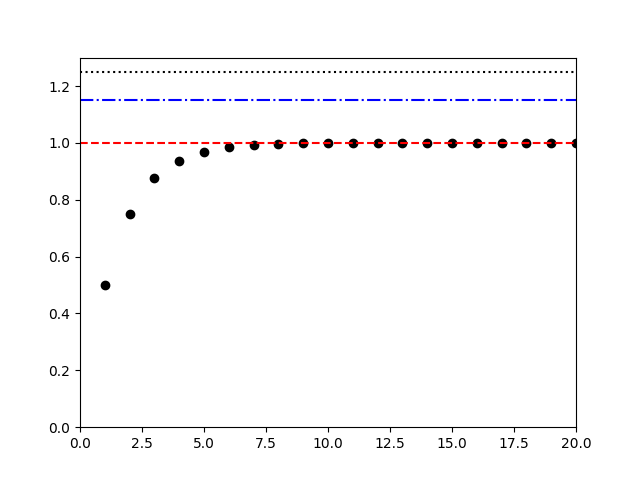
\includegraphics[width = 0.55\textwidth]{./assets/imgs/monotone_convergence.png}
\caption{Illustration de la convergence monotone avec la suite $x_n = 1 - 2^{-n}$. En rouge, on a la borne supérieure la plus petite possible ($B = 1$). En noir et bleu, on a des bornes supérieures plus grandes et donc non-optimales.}
\label{fig:conv_monotone}
\end{figure}

Maintenant, viennent les règles de calculs sur les limites. La première est la linéarité~:

\begin{greybox}
\textbf{Linéarité de la limite.} Soit $(x_n)$ et $(y_n)$ deux suites qui convergent avec limites respectives $\lim \limits_{n \to +\infty}x_n = x$ et $\lim \limits_{n \to +\infty}y_n = y$. Soit $\lambda, \mu \in \mathbb R$ deux nombres réels. Alors la suite $(z_n) = (\lambda \cdot x_n + \mu \cdot y_n)$ converge et sa limite vaut 
$$\lim \limits_{n \to +\infty}(\lambda \cdot x_n + \mu \cdot y_n) = \lambda \cdot \left(\lim \limits_{n \to +\infty}x_n\right) + \mu \cdot \left( \lim \limits_{n \to +\infty}y_n \right) = \lambda \cdot x + \mu \cdot y$$
\end{greybox}

Pour se convaincre de ce résultat, on peut utiliser le raisonnement (informel) suivant~: Lorsque $n$ est très grand, on a $x_n \approx x$, $y_n \approx y$ et donc $\lambda \cdot x_n + \mu \cdot y_n \approx \lambda \cdot x + \mu \cdot y$.

Le même raisonnement permet de se convaincre qu'on a le même comportement avec le produit ou quotient de deux suites convergentes.
\begin{greybox}
\textbf{Produit et quotient de limites.} Soit $(x_n)$ et $(y_n)$ deux suites qui convergent avec limites respectives $\lim \limits_{n \to +\infty}x_n = x$ et $\lim \limits_{n \to +\infty}y_n = y$. Alors~:

\begin{enumerate}
    \item La suite $(z_n) = (x_n \cdot y_n)$ converge et sa limite vaut $$\lim \limits_{n \to +\infty}(x_n \cdot y_n) = \left(\lim \limits_{n \to +\infty} x_n\right) \cdot \left(\lim \limits_{n \to +\infty} y_n\right) = x \cdot y$$
    \item Si $y,y_n \neq 0$ pour tout $n$, la suite $(z_n) = \left(\dfrac{x_n}{y_n}\right)$ converge et sa limite vaut $$\lim \limits_{n \to +\infty}\left( \frac{x_n}{y_n} \right) = \frac{\lim \limits_{n \to +\infty} x_n}{\lim \limits_{n \to +\infty} y_n} = \frac{x}{y}$$
\end{enumerate}
\end{greybox}

\section{Théorème des deux gendarmes}

Le théorème des deux gendarmes permet de déterminer la convergence d'une suite vers une limite $l \in \mathbb R$ grâce à la convergence de deux autres suites vers ce même nombre $l$.

Nous commençons par un cas particulier~:
\begin{boxthm}[Théorème des deux gendarmes : cas particulier]
Soient $(x_n)$ et $(y_n)$ deux suites et $l \in \mathbb R$. Supposons que $l \leq x_n \leq y_n$ pour tout $n$ et que la suite $(y_n)$ converge vers $l$. Alors la suite $(x_n)$ converge aussi vers $l$.
\label{thm:deux_gendarmes_part}
\end{boxthm}

La logique de ce théorème est assez similaire à celle du Théorème \ref{thm:conv_monotone} de convergence monotone. Dans le Théorème  \ref{thm:conv_monotone}, la croissance de la suite $(x_n)$ pousse la suite à converger vers la borne supérieure $B$ la plus petite. Dans notre situation, c'est la suite $(y_n)$ qui remplace la monotonie et va pousser la suite $(x_n)$ vers la borne inférieure $l$.

Du cas particulier, on peut déduire le cas général~:
\begin{boxthm}[Théorème des deux gendarmes]
Soient $(x_n)$, $(y_n)$, $(z_n)$ trois suites. Supposons que $y_n \leq x_n \leq z_n$ pour tout $n$ et que les suites $(y_n)$, $(z_n)$ convergent toutes deux vers une même limite $l \in \mathbb R$. Alors la suite $(x_n)$ converge aussi vers $l$.
\end{boxthm}

Ici, plutôt qu'avoir une borne inférieure fixe comme dans le Théorème \ref{thm:deux_gendarmes_part}, on a une autre suite qui pousse par le bas $(x_n)$ vers la limite $l \in \mathbb R$. Étant donné que $(x_n)$ est aussi poussée par le haut vers $l$, on obtient la convergence.

Comment déduit-on rigoureusement le cas général du cas particulier ? Par hypothèse, on a l'inégalité $0 \leq x_n - y_n \leq z_n - y_n$ pour tout $n$. De plus, $(z_n - y_n)$ converge vers $0$ par linéarité de la limite. Ainsi, le cas particulier implique que $(x_n - y_n)$ converge également vers $0$. En écrivant $x_n = y_n + (x_n - y_n)$, on obtient bien que $x_n$ converge vers $l$ (à nouveau par linéarité de la limite).

Finalement, terminons par un exemple d'application. Prenons la suite $x_n = \frac{\sin(n)}{n}$ pour $n \geq 1$. On se souvient que la fonction sinus donne toujours une valeur comprise entre $-1$ et $1$. Ainsi, on déduit l'inégalité
\[
-\frac{1}{n} \leq \frac{\sin(n)}{n} \leq \frac{1}{n} \quad \forall n \in \mathbb N^*
\]
Les suites $y_n = -\frac{1}{n}$ et $z_n = \frac{1}{n}$ convergent toutes deux vers $0$, donc il en va de même pour la suite $(x_n)$ grâce au Théorème des deux gendarmes.

\section{Théorème d'un gendarme}

Lorsqu'une suite diverge, on distingue un type de divergence particulier : la divergence vers l'infini.

\begin{boxdef}[Divergence d'une suite vers l'infini (informelle)]\label{def:divergence}
On dit qu'une suite $(x_n)_{n \geq 1}$ \emph{diverge vers} $+\infty$ si, en ignorant suffisamment de termes initiaux $x_1, x_2, ..., x_{n_0}$, \emph{tous} les éléments restant de la suite sont positifs et aussi grands que l'on veut. On note 
\[
\lim \limits_{n \to \infty} x_n \eqdef +\infty
\]
Similairement, on dit qu'une suite $(x_n)_{n \geq 1}$ \emph{diverge vers} $-\infty$ si, en ignorant suffisamment de termes initiaux $x_1, x_2, ..., x_{n_0}$, \emph{tous} les éléments restant de la suite sont négatifs et aussi grands (en valeur absolue) que l'on veut. On note 
\[
\lim \limits_{n \to \infty} x_n \eqdef -\infty
\]
\end{boxdef}

Malgré la notation, il faut se rappeler qu'une telle suite ne \textbf{converge pas}. De plus, une suite non-bornée \textbf{ne diverge pas forcément vers} $\pm \infty$ (prendre l'exemple $x_n = (-1)^n \cdot n$).

Un exemple typique de suite qui diverge vers $+\infty$ est donné par $x_n = n$ (ou $x_n = -n$ pour $-\infty$). En effet, si on se donne un $B > 0$ aussi grand que l'on veut, alors à partir de l'indice $n_0 = \lceil B \rceil$, on a $x_n > 0$ et $x_n > B$ pour tous les éléments restants de la suite. En fait, n'importe quelle suite donnée par un polynôme, i.e. $x_n = P(n)$ où $P(x)$ est un polynôme réel, diverge vers $\pm \infty$.

Toutefois, le Théorème \ref{thm:deux_gendarmes_part} est aussi valable, grâce au même raisonnement, pour les suites qui divergent vers l'infini~:

\begin{boxthm}[Théorème d'un gendarme]\label{thm:un_gendarme}
Soient $(x_n)$ et $(y_n)$ deux suites. 

Supposons que $x_n \leq y_n$ pour tout $n$ et que la suite $(y_n)$ diverge vers $-\infty$. Alors la suite $(x_n)$ diverge aussi vers $-\infty$.

Similairement, supposons que $y_n \leq x_n$ pour tout $n$ et que la suite $(y_n)$ diverge vers $+\infty$. Alors la suite $(x_n)$ diverge aussi vers $+\infty$.
\end{boxthm}
De ce théorème et de l'inégalité \ref{eq:fibonacci_lower_bound}, on déduit par exemple que la suite de Fibonacci diverge vers $+\infty$.

\section{Exemples de suites typiques}
Un cas particulier de suites qui revient souvent est la suite de la forme $x_n = \frac{P(n)}{Q(n)}$ où $P(n)$ et $Q(n)$ sont deux polynômes réels et $Q(n) \neq 0$ pour tout $n$. Par exemple, on pourrait avoir les suites
$$x_n = \frac{3n+1}{7n+2}, \quad y_n = \frac{5n^5 - 2n^2 + 9}{4n^3 + 100}, \quad z_n = \frac{8n^2 + n + 1}{12n^7 - 5n^5 + 3}$$
Dans ce genre de cas, la convergence de la suite ne dépend que des termes de plus haut degré des polynômes $P(n)$ et $Q(n)$. En effet, pour $n$ grand, les autres termes sont négligeables en comparaison des termes de plus haut degré (par exemple, $n^2$ est négligeable par rapport à $n^5$). On peut alors (informellement) écrire
$$x_n \approx \frac{3n}{7n} = \frac{3}{7}, \quad y_n \approx \frac{5n^5}{4n^3} = \frac{5n^2}{4}, \quad z_n \approx \frac{8n^2}{12n^7} = \frac{2}{3n^5} \approx 0$$
et cela permet de déterminer $\lim \limits_{n \to +\infty}x_n = \frac{3}{7}$, $\lim \limits_{n \to +\infty}y_n = +\infty$ et $\lim \limits_{n \to +\infty} z_n = 0$.

Un deuxième cas de suites fréquent est la suite géométrique de la forme $x_n = r^n$ pour $r \in \mathbb R$. On peut aussi la définir par récurrence : $x_1 = 1$ et $x_{n} = r x_{n-1}$ pour $n \geq 2$. On distingue plusieurs cas

\begin{enumerate}
    \item Si $r = 1$, il s'agit de la suite constante $x_n = 1$ qui converge vers $1$.
    \item Si $r = -1$, il s'agit de la suite alternée $x_n = (-1)^n$ qui est bornée, mais diverge.
    \item Si $0 \leq r < 1$, la suite est bornée, décroissante et donc elle converge vers un certain $l \in \mathbb R$. L'équation $x_n = r x_{n-1}$ pour tout $n \geq 2$ implique que la limite doit vérifier $l = r \cdot l$, ce qui ne laisse que la possibilité $l = 0$.
    \item Si $-1 < r \leq 0$, la suite se réécrit comme $x_n = (-1)^n |r|^n$ et vérifie
    $$-|r|^n \leq x_n \leq |r|^n$$
    où $0 \leq |r| < 1$ comme dans le cas précédant. La suite converge donc vers $0$ par le théorème des deux gendarmes, mais elle n'est ni croissante, ni décroissante.
    \item Si $r > 1$, la suite diverge vers $+\infty$. Il faut penser à une "croissance exponentielle" vers $+\infty$. Pour s'en convaincre mathématiquement, on peut par exemple prouver l'inégalité de Bernoulli : $r^n \geq 1 + n(r-1)$ lorsque $r > 1$.
    \item Si $r < 1$, la suite est non-bornée et change de signe constamment. Elle diverge. 
\end{enumerate}
